\chapter{Problemanalyse}

\section{Lægemiddelskift}
\textit{Hvad er et lægemiddelskift, hvorfor sker det og hvad medfører det?} \\
Udgifterne til sygehusmedicin er stigende i flere europæiske lande, hvorfor flere lægemidler substitueres, med henblik på at sænke udgifterne til medicin~\citep{Ess2003,Johnston2011}. Substitution af lægemidler betyder at et lægemiddel udskiftes til et andet lægemiddel enten ved generisk eller analog substitution~\citep{DanskSelskabforPatientsikkerhed2009, Kairi2017}. 

Generisk substitution er substitution af lægemidler, der er generisk ækvivalent med det foreskrevne lægemiddel, herunder samme aktive stof, identiske styrke, koncentration og administrationsvej~\citep{DanskSelskabforPatientsikkerhed2009, Kairi2017}. Generisk substitution medvirker til at lægemidlet skifter navn eller ændre varemærke~\citep{Kairi2017}. %Ulemperne ved generisk substitution er at selvom lægemidlet indeholder somme aktive stof kan producenten af lægemidlet anvende forskellige hjælpestoffer, som på trods af kliniske forsøg, kan vise signifikante forskelle for nogle patienter i forhold til interaktion af lægemidler og optagelse af lægemidlet. Derudover kan generisk substitution medføre at erstatningslægemidlet har et anderledes udseende som f.eks. form, størrelse og farve på dispenseringsformen, hvilket kan medvirke til at patienten mistænker en fejl ved ordinering og derved udelader at tage medicinen.~\citep{Kairi2017}

Analog substitution er substitutionen af et lægemiddel med et andet lægemiddel, der afviger i sammensætningen, men anses for at have lignende bivirkninger og terapeutiske egenskaber~\citep{DanskSelskabforPatientsikkerhed2009, Kairi2017}. Det vil sige at analog substitution er alle lægemidler som ikke opfylder generisk substitution.~\citep{Kairi2017}. %Foruden de ulemper som er beskrevet omkring generisk substitution kan analog substitution medvirke til at lægemidler inden for samme farmakologiske klasse afviger væsentligt fra deres biologiske virkning~\citep{Kairi2017}. Det er endnu ikke påvist hvilken betydning dette har for den terapeutiske virkning. Derudover har patientens holdning, accept og forståelse en betydning. Hvis patienten er fejlinformeret eller ikke har fået den rette information omkring analog substitution kan dette give et indtryk af utilstrækkelig eller uhensigtsmæssig behandling~\citep{Kairi2017}.


\section{Problemer ved lægemiddelskift} \label{sec:ProblemLaeg}
\textit{Hvilke problemer opstår ved lægemiddelskift og hvad skyldes disse problemer?}

Lægemiddelskift medfører substitution af lægemidler, hvilket betyder at et lægemiddel udskiftes til et andet enten ved generisk eller analog substitution. Generisk substitution er substitution af lægemidler, der er generisk ækvivalent med det foreskrevne lægemiddel, herunder samme aktive stof, identiske styrke, koncentration og administrationsvej~\citep{DanskSelskabforPatientsikkerhed2009, Kairi2017}. Generisk substitution medvirker til at lægemidlet skifter navn eller ændre varemærke~\citep{Kairi2017}. Analog substitution er substitutionen af et lægemiddel med et andet lægemiddel, der afviger i sammensætningen, men anses for at have lignende bivirkninger og terapeutiske egenskaber~\citep{DanskSelskabforPatientsikkerhed2009, Kairi2017}. Det vil sige at analog substitution er alle lægemidler som ikke opfylder generisk substitution.~\citep{Kairi2017}.

Substitution her forskellige ulemper som kan lede til patientsikkerhedsmæssige konsekvenser~\citep{DanskSelskabforPatientsikkerhed2009}. Ved generisk substitution kan producenten af lægemidlet anvende forskellige hjælpestoffer, som på trods af kliniske forsøg, kan vise signifikante forskelle for nogle patienter i forhold til optagelse og interaktion af lægemidler~\citep{Kairi2017}. Derudover kan generisk substitution medføre at erstatningslægemidlet har ændret form, størrelse eller farve, hvormed fejl ved ordinering mistænkes og patienten derved udelader at tage medicinen~\citep{Kairi2017}. Foruden de beskrevne ulemper ved generisk substitution kan analog substitution medvirke til at lægemidler inden for samme farmakologiske klasse afviger væsentligt fra deres biologiske virkning~\citep{Kairi2017}. Det er endnu ikke påvist hvilken betydning dette har for den terapeutiske virkning. Derudover har patientens holdning, accept og forståelse en betydning. Hvis patienten er fejlinformeret eller ikke har fået den rette information omkring analog substitution kan dette give et indtryk af utilstrækkelig eller uhensigtsmæssig behandling~\citep{Kairi2017}. 

Et norsk studie har undersøgt konsekvenserne ved generisk substitution~\citep{Hakonsen2010}. Interview med 100 sygeplejersker påviste at der opstod fejlmedicinering ved generiske lægemidler~\citep{Hakonsen2010}. Ud af disse følte 92~\% af sygeplejerskerne at generiske lægemidler var tidskrævende og 91~\% at risikoen for fejl øges ved dispensering af disse, hvoraf 42~\% oplevede fejl som følge af generisk substitution~\citep{Hakonsen2010}.
Medicineringsfejl ved generisk substitution fremgår af Figur \ref{fig:GeneriskSubstitution}.

\begin{figure}[H]\centering	\includegraphics[width=1\textwidth]{billeder/GenSub.png} 
	\caption{Medicineringsfejl ved generisk substitution rapporteret (n=100)~\citep{Hakonsen2010}.}
	\label{fig:GeneriskSubstitution}  
\end{figure}

Det fremgår af Figur \ref{fig:GeneriskSubstitution} at størstedelen af fejlmedicinering ved generisk substitution skyldes forkert lægemiddel, hvoraf en mindre del skyldes forkert formulering og i sjældnere tilfælde forkert dosis, administrationsvej og udeladelse af dosis. Forkert lægemiddel forstås som at et andet lægemiddel end det oprindelige er dispenseret. Formulering beskriver lægemidlet fysiske form som f.eks. tabelletform, dosis beskriver mængden af lægemidlet og administrationsvej beskriver hvordan indgiften af et lægemiddel tages f.eks. via munden.

Det norske studie undersøgte ligeledes årsagerne til medicineringsfejl, hvilket er rapporteret af 42 sygeplejersker~\citep{Hakonsen2010} og fremgår af Figur \ref{fig:GeneriskSubstitution1}.

\begin{figure}[H]\centering	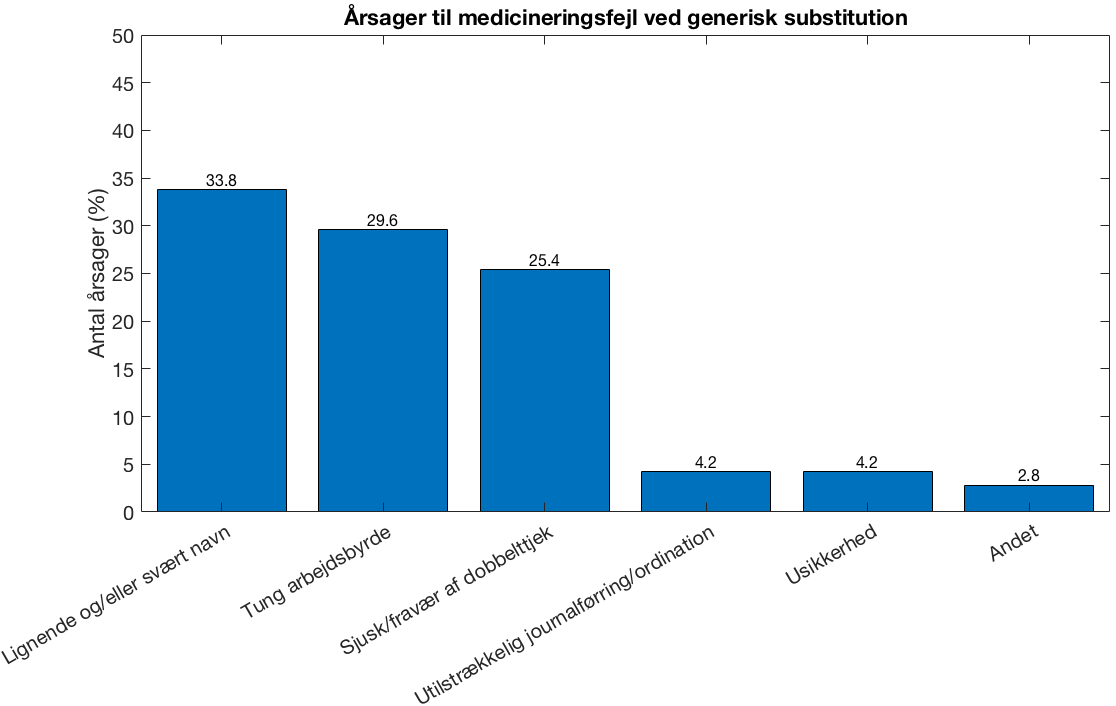
\includegraphics[width=1\textwidth]{billeder/GenSub1.png} 
	\caption{Årsager til medicineringsfejl ved generisk substitution (n=42)~\citep{Hakonsen2010}.}	\label{fig:GeneriskSubstitution1}  
\end{figure}

Af Figur \ref{fig:GeneriskSubstitution1} fremgår det at størstedelen af årsagerne til medicineringsfejl ved generisk substitution skyldes lignende og/eller vanskeligt lægemiddelnavn, kraftig arbejdsbyrde og sløvhed eller fravær af dobbelttjek. En mindre del skyldes utilstrækkeligt journalførring og/eller ordination, usikkerhed eller andet. 

I flere lande, inklusiv Danmark, opstår forkert lægemiddel ofte i forbindelse med forvirring ved forveksling af navn eller emballage~\citep{DanskSelskabforPatientsikkerhed2009}, hvilket afspejles i det norske studie. Forveksling af lægemiddelnavne har i sjældnere tilfælde haft konsekvenser som har medført forlænget indlæggelse, forværret sygdom eller dødsfald.~\citep{DanskSelskabforPatientsikkerhed2009}

Forveksling af navn kan for eksempel forekomme ved panodil, som er et smertestillende lægemiddel, og plendil, som anvendes til behandling af forhøjet blodtryk~\citep{DanskSelskabforPatientsikkerhed2009}. Derudover kan forskellige suffiks eller præfiks skabe forvirring og give anledning til fejl dispensering såsom Efexor kontra Efexor Depot~\citep{DanskSelskabforPatientsikkerhed2009} Udover selve lægemidlets navn kan lægemidler som har lignede navne, så kaldte look-a-like, prædisponeres til medicineringsfejl som kan have patientsikkerhedsmæssige konsekvenser~\citep{Wittich2014}. Eksempler på look-a-like lægemidler er  dopamin og dobutamin~\citep{Wittich2014}. Brugen af forkortelser i ordinationen eller kommunikation medfører ligeledes til øget risiko for medicineringsfejl~\citep{Wittich2014}.

Nogle af sygeplejerskerne i det norske studie mente at forvirringen over at finde den korrekte substitution kunne lede til at doseringen og formulationen var skyld i medicineringsfejl~\citep{Hakonsen2010}. Kognitive forstyrrelser, som fejl ved bekræftelse eller mangel på situationsfornemmelse, kan bidrage til medicineringsfejl. Et eksempel på dette kan være forvirring over at lægemidlets leverandør ændres hyppigt, hvormed det nuværende lægemidlet substitueres til et andet~\citep{Wittich2014}

I takt med at hospitalets medicin opgørelse gennemgår ændringer jævnligt og antallet af generiske substitutioner stiger medvirker dette til at arbejdsbyrden er steget~\citep{Hakonsen2010}. Til trods for at sygeplejerskernes arbejde er blevet mere kompleks og krævende har de kun modtaget en begrænset oplæring inden for området.~\citep{Hakonsen2010}.

Medicinering var den hyppigste årsag til rapportering af utilsigtede hændelser i Danmark i år 2013~\citep{Patientombuddet2013}. Antallet af rapporteringer i Region Nordjylland er steget med over 36~\% fra år 2012 til 2014~\citep{Jensen2014}. Ud af 824 rapporterede utilsigtede hændelser i år 2014 skyldes 97\% medicinering, 86\% administration af medicin og 41\% disponering~\citep{Jensen2014}, hvor mere end én rapporteret utilsigtede hændelser kan skyldes en eller flere grunde.  Håndteringen af medicin er kompleks, da det er en mangeartet proces som involverer flere personer og mange led. I alle led blev der påvist fejl~\citep{Barker2002,Sundhedsstyrelsen2005, Lisby2005, Tully2009}.Størstedelen af fejl forekommer i forbindelse med ordination og administration og en mindre andel af fejl ved transskribering og dispensering~\citep{Agrawal2009, Anderson2002} En fælles årsag i disse studier var forkert dosis, forkert lægemiddel og udeladelse af henholdsvis ordination, dispensering og administration~\citep{Barker2002,Sundhedsstyrelsen2005,Lisby2005, Tully2009}.
%Størstedelen af medicineringsfejl ved ordination inkluderer brug af forkert lægemiddel, doseringsform, styrkeberegning, manglende kontrol af allergier og manglende evne til at justere doseringen hos patienter med nedsat nyre- eller leverfunktion.~\citep{Agrawal2009}.


\section{Implementering af lægemiddelskift}
\textit{Hvilken proces gennemgår lægemiddelskift før det når til klnikken og hvilke ulemper er forbundet med denne proces?}

%I Danmark sendes lægemidler i udbud af Amgros, som står for indkøb af lægemidler til de offentlige danske hospitaler, med henblik på at begrænse udgifterne til sygehusmedicin~\citep{Amgros2018b}. Størstedelen af lægemidler sendes i udbud en gang årligt fra start september til midt november~\citep{Sygehusapoteket2017}. Hvis en ny lægemiddelvirksomhed vinder leverancen af et lægemiddel indgås et kontraktskift, hvilket medvirker til substitution af lægemidler~\citep{Amgros2015}. 

%Indkøb af lægemidler til distribution til de offentlige danske hospitaler foretages i Danmark af sygehusapoteker som er placeret i de enkelte regioner.

For at forebygge fejlmedicinering og forbedre patientsikkerheden ved lægemiddelskift formidler Sygehusapoteket Region Nordjylland (SRN) information om lægemiddelskiftene til de enkelte hospitalsafdelinger i regionen inden lægemidlet implementeres i klinikken. Hospitalsafdelingerne informeres om lægemiddelskift via LægemiddelNyt som har til hensigt at gøre klinikken opmærksom på komplekse lægemiddelskift. Udarbejdelsen af LægemiddelNyt og vurdering af kompleksiteten af lægemiddelskift foretages af ATC-ansvarlige medarbejdere fra SRN. Denne vurderingen sker på baggrund af ændringer i lægemidlets navn, dispenseringsform og styrke samt den ATC-ansvarlige medarbejders tidligere erfaring, retningslinjer, indsamlede problemstillinger og indsamlet viden. Denne proces er erfaringsbaseret og udføres manuelt, hvilket gør processen  sårbar og personafhængig. 


%For at forebygge problemer som kan opstå i klinikken vurderer ATC-ansvarlige medarbejdere i SRN kompleksiteten af lægemiddelskift før dette implementeres i klinikken. Vurderingen af lægemiddelskift sker på baggrund af ATC-ansvarlige medarbejders tidligere erfaringer, retningslinjer, indsamlede problemstillinger vedrørerende lægemiddelskift, viden indsamlet samt ændringer ved lægemidlet som navn, dispenseringsform og styrke. Disse risikofaktorer vægtes af de ATC-ansvarlige medarbejdere, hvormed processen er sårbar, da den er personafhængig og manuel samt stiller krav til den enkelte medarbejders viden og erfaring inden for området. 

\section{Forebyggelse af problemstillinger ved lægemiddelskift}
\textit{hvilke teknologier anvendes til at forbygge medicineringsfejl og hvordan kan den nuværende vurdering af lægemiddel optimeres?} \\
Flere studier har påvist at informationssystemer er anvendelige til forebyggelsen af fejlmedicinering ved ordination, dispensering og administration~\citep{Agrawal2009, Anderson2002}. Et eksempel er computerbaseret ordineringssystemer, som anvendes til at strukturere ordre, gøre disse letlæselige og fuldkommen samt gøre nødvendige oplysninger tilgængelige for klinikeren~\citep{Agrawal2009,Bates2000a}. I en kombination med beslutningsstøtte system, som f.eks. interaktion mellem lægemidler og automatisk beregning af styrke ved ændring i denne~\citep{Agrawal2009}, har computerbaseret ordineringssystem påvist at være effektiv i forbedring af patientsikkerheden~\citep{Agrawal2009, Bates2000a}. Samme effekt er påvist for systemer med begrænset brug af beslutningsstøtte~\citep{Bates2000a}. Til dispensering anvendes forskellige teknologier som f.eks. robotter og automatiserede skabe, som anvender stregkoder til at genkende medicin, hvilket medvirker til at reducere antallet af fejl relateret til emballage og dispensering.~\citep{Agrawal2009}

Fælles for de ovenstående informationssystemer er at de anvendes i klinikken når lægemiddelskiftet er implementeret. Ingen videnskabelig litteratur har undersøgt om informationssystemer kan anvendes til at opnå en effektiv implementering af lægemiddelskift i klinikken og derved gøre den nuværende vurdering mindre personafhængig og sårbar. Da informationssystemer,modsat den menneskelige evne, er i stand til at organisere og identificere sammenhænge mellem informationer fra en større mængde af data, vil et system som dette medvirke til at processen blev ensartet og derved mindre personafhængig. Derudover vil flere risikofaktorer forbundet med lægemiddelskift tages med i vurderingen, hvilket vil understøtte beslutningen.  

Informationssystemer er bredt anvendt til risikovurderingen\citep{}. Disse systemer anvender ofte statistisk 
..... Bla Bla.. 




Ved anvendelsen af machine learning skal risikovurdering målrettes problemer med medicinen, men da data ikke er til rådighed er dette ikke muligt. Man kan vælge statistisk eller regelbaseret tilgang..


Machine learning så man målretter det til problemet med medicin, men der er ikke data til at lave dette. Hvilke teknologier findes, hvilke lignende teknologier findes – der mangler stadig eksempler, det behøver ikke at være nogle som er matchet fuldstændig, risikoscore, beslutningsstøttesystemer. Givet vi har disse erfaringer og kender processerne og tilgængeligt materiale – vælge en teknologi.
Man kan vælge statistisk eller regelbaseret kan man gå den og den vej, hvis det er statistisk, har man brug for …. Den samme vej og det og det data..




